\documentclass{ajc}
\usepackage[output-decimal-marker={,},per-mode=fraction,fraction-function=\tfrac]{siunitx}
\mathcode`,="002C
\numberwithin{equation}{subsection}
\newcommand\numberthis{\addtocounter{equation}{1}\tag{\theequation}}


\title{Mathe}
\author{Alexander Jacob}
\date{Schuljahr 2024/2025}

\begin{document}
	\section{Vektoren}
	
	\subsection{Spurpunkte berechnen}
	\paragraph{a)} Bestimmen Sie die Spurpunkte der Geraden
	\begin{equation}
		\mathbf{g}: \overrightarrow{x}=\left(\begin{array}{r} 2 \\ 1 \\ 7\end{array}\right) + \lambda \cdot \left(\begin{array}{r} 0 \\ 6 \\ 4\end{array}\right) \text{\quad und \quad} \mathbf{h}: \overrightarrow{x}=\left(\begin{array}{r} -3 \\ 0 \\ -5\end{array}\right) + \mu \cdot \left(\begin{array}{r} 1 \\ 3 \\ 2\end{array}\right). 
	\end{equation}
	
	\subparagraph{zu g:}
	\begin{equation}
		\overrightarrow{x}=\left(\begin{array}{r} 2 \\ 1 + 6\lambda \\ 7 + 4\lambda \end{array}\right)
	\end{equation}
	
	Bedingung für Spurpunkt mit $x_1\text{-}x_2$-Ebene:\quad $x_3 = 0$
	
	Punkt von \textbf{g} in der $x_1\text{-}x_2$-Ebene:\quad $x_3 = 0 \Leftrightarrow 0 = 7 + 4\lambda \Leftrightarrow \lambda = -\frac{7}{4}$
	
	Ortsvektor des Spurpunkts: 
	\begin{equation}
	\overrightarrow{s_\text{12}}=\left(\begin{array}{r} 2 \\ -9,5 \\ 0\end{array}\right)
	\end{equation}
	Spurpunkt: $S_\text{12}(2|-9,5|0)$
	
	Bedingung für Spurpunkt mit $x_1\text{-}x_3$-Ebene:\quad $x_2 = 0$
	
	Punkt von \textbf{g} in der $x_1\text{-}x_3$-Ebene:\quad $x_2 = 0 \Leftrightarrow 0 = 1 + 6\lambda \Leftrightarrow \lambda = -\frac{1}{6}$
	
	Ortsvektor des Spurpunkts: 
	\begin{equation}
		\overrightarrow{s_\text{13}}=\left(\begin{array}{r} 2 \\ 0 \\ 6,\overline{3}\end{array}\right)
	\end{equation}
	Spurpunkt: $S_\text{12}(2|0|6,\overline{3})$
	
	Bedingung für Spurpunkt mit $x_2$-$x_3$-Ebene:\quad $x_1 = 0$
	
	Punkt von \textbf{g} in der $x_2\text{-}x_3$-Ebene:\quad $x_1 = 0 \Leftrightarrow 0 \ne 2 \,\lightning$
	
	Es gibt keinen Spurpunkt von $g$ in der $x_2\text{-}x_3$-Ebene.
	
	\subparagraph{zu h:}
	\begin{equation}
		\overrightarrow{x}=\left(\begin{array}{r} -3 + \mu \\ 3\mu \\ -5 + 2\mu\end{array}\right)
	\end{equation}
	
	Bedingung für Spurpunkt mit $x_1\text{-}x_2$-Ebene:\quad $x_3 = 0$
	
	Punkt von \textbf{h} in der $x_1\text{-}x_2$-Ebene:\quad $x_3 = 0 \Leftrightarrow 0 = -5 + 2\mu \Leftrightarrow \mu = \frac{5}{2}$
	
	Ortsvektor des Spurpunkts: 
	\begin{equation}
		\overrightarrow{s_\text{12}}=\left(\begin{array}{r} -0,5 \\ 7,5 \\ 0\end{array}\right)
	\end{equation}
	Spurpunkt: $S_\text{12}(-0,5|7,5|0)$
	
	Bedingung für Spurpunkt mit $x_1\text{-}x_3$-Ebene:\quad $x_2 = 0$
	
	Punkt von \textbf{h} in der $x_1\text{-}x_3$-Ebene:\quad $x_2 = 0 \Leftrightarrow 0 = 3\mu \Leftrightarrow \mu = 0$
	
	Ortsvektor des Spurpunkts: 
	\begin{equation}
		\overrightarrow{s_\text{13}}=\left(\begin{array}{r} -3 \\ 0 \\ -5\end{array}\right)
	\end{equation}
	Spurpunkt: $S_\text{12}(-3|0|-5)$
	
	Bedingung für Spurpunkt mit $x_2$-$x_3$-Ebene:\quad $x_1 = 0$
	
	Punkt von \textbf{h} in der $x_2\text{-}x_3$-Ebene:\quad $x_1 = 0 \Leftrightarrow 0 = -3 + \mu \Leftrightarrow \mu = 3$
	
	Ortsvektor des Spurpunkts: 
	\begin{equation}
		\overrightarrow{s_\text{23}}=\left(\begin{array}{r} 0 \\ 9 \\ 1\end{array}\right)
	\end{equation}
	Spurpunkt: $S_\text{23}(0|9|1)$
	
	
	\paragraph{b)} Von einer Geraden sind die Spurpunkte $S_\text{12} (2|3|0)$ und \linebreak $S_\text{23} (0|-1|1)$ bekannt. Bestimmen Sie den Spurpunkt $S_\text{13}$.
	
	Zweipunktegleichung einer Geraden:
	\begin{equation}\label{eq:1.1zpg}
		\mathbf{g}: \overrightarrow{x}= \vec{a} + \lambda \cdot \left(\overrightarrow{b} - \overrightarrow{a}\right)
	\end{equation}
	
	Mit den eingesetzten Punkten $S_\text{12}$ und $S_\text{23}$ in \ref{eq:1.1zpg} ergibt sich:
	\begin{equation}\label{eq:1.1zpg_ein}
		\mathbf{g}: \overrightarrow{x}= \left(\begin{array}{r} 2 \\ 3 \\ 0\end{array}\right) + \lambda \cdot \left(\begin{array}{r} -2 \\ -4 \\ 1\end{array}\right) = \left(\begin{array}{r} 2 - 2\lambda \\ 3 - 4\lambda \\ \lambda\end{array}\right)
	\end{equation}
	
	Bedingung für Spurpunkt mit $x_1\text{-}x_3$-Ebene:\quad $x_2 = 0$
	
	Punkt von \textbf{g} in der $x_1\text{-}x_3$-Ebene:\quad $x_2 = 0 \Leftrightarrow 0 = 3 - 4\lambda \Leftrightarrow \lambda = \frac{3}{4}$
	
	Ortsvektor des Spurpunkts: 
	\begin{equation}
		\overrightarrow{s_\text{13}}=\left(\begin{array}{r} 0,5 \\ 0 \\ 0,75\end{array}\right)
	\end{equation}
	Spurpunkt: $S_\text{12}(0,5|0|0,75)$
	
	\subsection{Pyramide}
	Gegeben ist eine gerade Pyramide mit quadratischer Grundfläche. Die Seitenlänge des in der $x_1$-$x_2$-Ebene liegenden Quadrates ABCD beträgt 80 m, die Pyramide hat eine Höhe von 60 m.
	
	Die Richtung der einfallenden Sonnenstrahlen ist gegeben durch den Vektor $\overrightarrow{u}=\left(\begin{array}{r} 2 \\ 4 \\ -3\end{array}\right)$.
	
	Der Schattenpunkt $S'$ der Pyramidenspitze $S$ liegt in der $x_1$-$x_2$-Ebene.
	Berechnen Sie die Koordinaten von $S'$.
	
	\begin{figure}[ht]
		\centering
		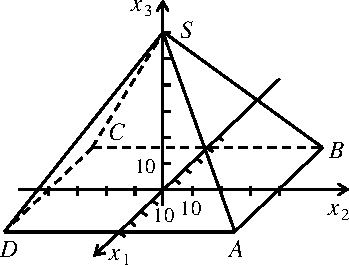
\includegraphics[width=0.5\textwidth]{ma_002_pyramide.pdf}
		\caption{Skizze der Pyramide.}
		\label{fig:002_pyramide}
	\end{figure}

	Vektor der auf Punkt $S$ fallenden Sonnenstrahlen:
	\begin{equation}
		\overrightarrow{x}=\left(\begin{array}{r} 0 \\ 0 \\ 60\end{array}\right) + \lambda \cdot \left(\begin{array}{r} 2 \\ 4 \\ -3\end{array}\right)
	\end{equation}
	
	Bedingung für Spurpunkt mit $x_1$-$x_2$-Ebene:\quad $x_3 = 0$

	Punkt in der $x_1$-$x_2$-Ebene: $0 = 60 -3 \lambda \Leftrightarrow 60 = 3\lambda \Leftrightarrow \lambda = 20$
	
	Schattenpunkt: $S'(40|80|0)$
	
	\subsection{Schatten einer Plakatwand}
	Vor einem Haus steht eine Plakatwand, die \SI{3}{\m} breit und \SI{6}{m} hoch ist. Ein Punkt der Wand ist $A(6|2|6)$. Auf die Plakatwand fällt paralleles Sonnenlicht. Die Richtung der Sonnenstrahlen ist gegeben durch den Vektor
	\begin{equation*}
		\overrightarrow{u}=\left(\begin{array}{r} -3 \\ 1 \\ -1\end{array}\right).
	\end{equation*}
	Bestimmen und beschreiben Sie den Verlauf des Schattens an der Hauswand und auf dem Boden.
	
	\begin{figure}[ht]
		\centering
		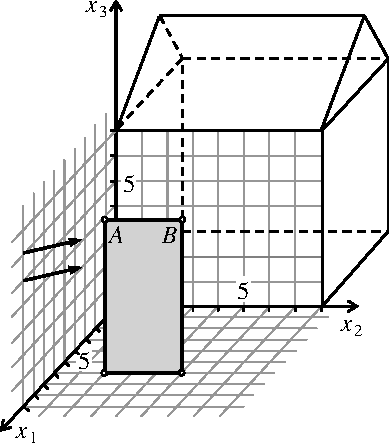
\includegraphics[width=0.5\textwidth]{ma_001_schatten.pdf}
		\caption{Skizze der Plakatwand mit Hauswand.}
		\label{fig:001_schatten}
	\end{figure}
	
	Geraden in Richtung des Sonneneinfalls:
	\begin{equation}
		\mathbf{g}: \overrightarrow{x}=\left(\begin{array}{r} 6 \\ 2 \\ 6\end{array}\right) + \lambda \cdot \left(\begin{array}{r} -3 \\ 1 \\ -1\end{array}\right) = \left(\begin{array}{r} 6 - 3 \lambda \\ 2 + \lambda \\ 6 - \lambda\end{array}\right)
	\end{equation}
	\begin{equation}
		\mathbf{h}: \overrightarrow{x}=\left(\begin{array}{r} 6 \\ 5 \\ 6\end{array}\right) + \mu \cdot \left(\begin{array}{r} -3 \\ 1 \\ -1\end{array}\right) = \left(\begin{array}{r} 6 - 3 \mu \\ 5 + \mu \\ 6 - \mu\end{array}\right)
	\end{equation}
	
	Gesucht sind jeweils die Spurpunkte von \textbf{g} und \textbf{h} mit der $x_2\text{-}x_3$-Ebene (= Hauswand).
	
	Bedingung für Spurpunkt mit $x_2$-$x_3$-Ebene:\quad $x_1 = 0$
	
	\paragraph{Für g gilt:} 
	
	Punkt von \textbf{g} in der $x_2\text{-}x_3$-Ebene:\quad $x_1 = 0 \Leftrightarrow 0 = 6 - 3 \lambda \Leftrightarrow \lambda = 2$
	
	Ortsvektor des Spurpunkts: 
	\begin{equation}
		\overrightarrow{s_\text{A23}}=\left(\begin{array}{r} 0 \\ 4 \\ 4\end{array}\right)
	\end{equation}
	Spurpunkt: $S_\text{23}(0|4|4)$
	
	\paragraph{Für h gilt:} 
	
	Punkt von \textbf{h} in der $x_2\text{-}x_3$-Ebene:\quad $x_1 = 0 \Leftrightarrow 0 = 6 + -3 \mu \Leftrightarrow \mu = 2$
	
	Ortsvektor des Spurpunkts: 
	\begin{equation}
		\overrightarrow{s_\text{B23}}=\left(\begin{array}{r} 0 \\ 7 \\ 4\end{array}\right)
	\end{equation}
	Spurpunkt: $S_\text{B23}(0|7|4)$
	
	Der Schatten der Plakatwand fällt also zum Teil auf die Hauswand bis auf eine Höhe von \SI{4}{\meter} mit einer Breite von \SI{3}{\meter}. Der andere Teil des Schattens fällt demnach auf den Boden vor der Hauswand zwischen den Punkten $A_0$, $B_0$, $S_{A0}$ und $S_{B0}$. Für diese Punkte gilt, dass sie senkrecht unter den Punkten $A$, $B$, $S_\text{A23}$ und $S_\text{B23}$ auf der $x_1\text{-}x_2$-Ebene liegen. Es gilt: $A_0 = (6|2|0)$, $B_0 = (6|5|0)$, $S_{A0} = (0|4|0)$ und $S_{B0} = (0|7|0)$.
	
	\subsection{Lageuntersuchung von Geraden}
	Untersuchen Sie die Geraden \textbf{g} und \textbf{h} auf ihre gegenseitige Lage. Berechnen Sie gegebenenfalls den Schnittpunkt.
	
	\begin{equation}
		\mathbf{g}: \overrightarrow{x}=\left(\begin{array}{r} -11 \\ 9 \\ 1\end{array}\right) + \lambda \cdot \left(\begin{array}{r} -4 \\ 3 \\ -2\end{array}\right) \text{\quad ; \quad} \mathbf{h}: \overrightarrow{x}=\left(\begin{array}{r} -4 \\ 11 \\ 4\end{array}\right) + \mu \cdot \left(\begin{array}{r} 3 \\ 5 \\ 1\end{array}\right)
	\end{equation}
	
	\begin{itemize}
		\item \textit{Test auf Parallelität} \\ 
		Die Richtungsvektoren sind nicht kollinear, daher sind die Geraden nicht parallel.
		
		\item \textit{Lageentscheidung (Gleichsetzungsverfahren)} \\
		\begin{alignat*}{2}
			\left(\begin{array}{r} -11 \\ 9 \\ 1\end{array}\right) + \lambda \cdot \left(\begin{array}{r} -4 \\ 3 \\ -2\end{array}\right) &= \left(\begin{array}{r} -4 \\ 11 \\ 4\end{array}\right) + \mu \cdot \left(\begin{array}{r} 3 \\ 5 \\ 1\end{array}\right) \\
			&\iff \left(\begin{aligned} -4 \lambda - 3 \mu &= 7 \\ 3 \lambda - 5 \mu &= 2 \\ -2 \lambda  - 1 \mu &= 3 \end{aligned}\right) \begin{array}{c} \text{(I)} \\ \text{(II)} \\ \text{(III)}\end{array} \numberthis
		\end{alignat*}
		
		Lösung: $\begin{array}{l}
			3\cdot\text{(III)} - \text{(I)}: \quad -2\lambda = 2 \Leftrightarrow \lambda = -1 \\ \text{Einsetzen in (III)}: \quad 2 - \mu = 3 \Leftrightarrow \mu = -1 \\ \text{Probe in  (I)}: \quad -4\cdot(-1) -3\cdot(-1) = 7 \checkmark \end{array}$
			
		Das Gleichungssystem ist für $\lambda = -1$ und $\mu = -1$ erfüllt, somit gibt es einen Schnittpunkt. \\
		\item \textit{Schnittpunktberechnung} \\
		$\lambda$ in $g$ eingesetzt gibt: 
		\begin{equation}
			\overrightarrow{x}=\left(\begin{array}{r} -11 \\ 9 \\ 1\end{array}\right) -1 \cdot \left(\begin{array}{r} -4 \\ 3 \\ -2\end{array}\right) = \left(\begin{array}{r} -7 \\ 6 \\ 3\end{array}\right)
		\end{equation}
		Die Geraden scheiden sich im Punkt $S(-7|6|3)$.
	\end{itemize}
	
	\subsection{Flugzeugcrash}
	Ein Passagierflugzeug $\text{F}_1$ befindet sich im Punkt  $A(10|30|2)$ und fliegt geradlinig in Richtung des Punktes $B(40|90|2)$. Ein Sportflugzeug $\text{F}_2$ befindet sich zum gleichen Zeitpunkt im Punkt $C(70|90|11)$ und nimmt Kurs auf den Punkt $D(70|110|8)$ (alle Angaben in km).
	
	\paragraph{a)} Begründen Sie, dass sich die beiden Flugzeuge auf Kollisionskurs befinden.
	
	\subparagraph{zu $\text{F}_1$} Mit den eingesetzten Punkten $A$ und $B$ in die Zweipunktegleichung \ref{eq:1.1zpg} ergibt sich: 
	\begin{equation}
		\mathbf{F_1}: \overrightarrow{x}=\left(\begin{array}{r} 10 \\ 30 \\ 2\end{array}\right) + \lambda \cdot \left(\begin{array}{r} 30 \\ 60 \\ 0\end{array}\right)
	\end{equation}
	
	\subparagraph{zu $\text{F}_2$} Mit den eingesetzten Punkten $C$ und $D$ in die Zweipunktegleichung \ref{eq:1.1zpg} ergibt sich: 
	\begin{equation}
		\mathbf{F_2}: \overrightarrow{x}=\left(\begin{array}{r} 70 \\ 90 \\ 11\end{array}\right) + \mu \cdot \left(\begin{array}{r} 0 \\ 20 \\ -3\end{array}\right)
	\end{equation}
	
	\begin{itemize}
		\item \textit{Test auf Parallelität} \\ 
		Die Richtungsvektoren sind nicht kollinear, daher sind die Geraden nicht parallel.
		
		\item \textit{Lageentscheidung (Gleichsetzungsverfahren)} \\
		\begin{alignat*}{2}
			\left(\begin{array}{r} 10 \\ 30 \\ 2\end{array}\right) + \lambda \cdot \left(\begin{array}{r} 30 \\ 60 \\ 0\end{array}\right) &= \left(\begin{array}{r} 70 \\ 90 \\ 11\end{array}\right) + \mu \cdot \left(\begin{array}{r} 0 \\ 20 \\ -3\end{array}\right) \\
			&\iff \left(\begin{aligned} 30 \lambda &= 60 \\ 60 \lambda - 20 \mu &= 60 \\ -3 \mu &= 9 \end{aligned}\right) \begin{array}{c} \text{(I)} \\ \text{(II)} \\ \text{(III)}\end{array} \numberthis
		\end{alignat*}
		
		Lösung: $\begin{array}{l}
			\text{(I) nach } \lambda: \quad 30 \lambda = 60 \Leftrightarrow \lambda = 2 \\ \text{(III) nach } \mu: \quad 3\mu = 9 \Leftrightarrow \mu = 3 \\ \text{Probe in  (II)}: \quad 60\cdot2 -20\cdot3 = 60 \checkmark \end{array}$
		
		Das Gleichungssystem ist für $\lambda = 2$ und $\mu = 3$ erfüllt, somit gibt es einen Schnittpunkt.
		
		\item \textit{Schnittpunktberechnung} \\
		$\lambda$ in $\text{F}_1$ eingesetzt gibt: 
		\begin{equation}
			\overrightarrow{x}=\left(\begin{array}{r} 10 \\ 30 \\ 2\end{array}\right) + 2 \cdot \left(\begin{array}{r} 30 \\ 60 \\ 0\end{array}\right) = \left(\begin{array}{r} 70 \\ 150 \\ 2\end{array}\right)
		\end{equation}
		Die Flugzeuge kollidieren im Punkt $S(70|150|2)$.
	\end{itemize}
	
	\paragraph{b)} Prüfen Sie, ob es tatsächlich zum Crash kommt, wenn sich $\text{F}_1$ mit der Geschwindigkeit 800 km/h, $\text{F}_2$ mit 350 km/h bewegt.
	
	Verbindungsvektor zwischen $A$ und $S$:
	\begin{equation}
		\overrightarrow{f_1} = \left(\begin{array}{r} 70 - 10 \\ 150 - 30 \\ 2 - 2\end{array}\right) = \left(\begin{array}{r} 60 \\ 120 \\ 0\end{array}\right) 
	\end{equation}
		
	Länge des Verbindungsvektors zwischen $A$ und $S$:
	\begin{equation}
		\left|\overrightarrow{f_1}\right| = \sqrt{60^2 + 120^2 + 0^2} = \SI{134,16}{km}
	\end{equation}
	
	Zeit bis zum Eintreffen:
	\begin{equation}
		\frac{\SI{134,16}{km}}{\SI{800}{\km\per\hour}} = \SI{0,1677}{\hour}
	\end{equation}
	
	Verbindungsvektor zwischen $C$ und $S$:
	\begin{equation}
		t_1 = \overrightarrow{f_2} = \left(\begin{array}{r} 70 - 70 \\ 150 - 90 \\ 2 - 11\end{array}\right) = \left(\begin{array}{r} 0 \\ 60 \\ -9\end{array}\right) 
	\end{equation}
	
	Länge des Verbindungsvektors zwischen $C$ und $S$:
	\begin{equation}
		\left|\overrightarrow{f_2}\right| = \sqrt{0^2 + 60^2 + (-9)^2} = \SI{60,67}{km}
	\end{equation}
	
	Zeit bis zum Eintreffen:
	\begin{equation}
		t_2 = \frac{\SI{60,67}{km}}{\SI{350}{\km\per\hour}} = \SI{0,1733}{\hour}
	\end{equation}
	
	Es kommt vermutlich zum Crash, weil beide Flugzeuge zu einem sehr ähnlichen Zeitpunkt im Punkt $S$ eintreffen werden.
	
\end{document}